\section{The Minimum Shared Multicast Tree Problem}
\label{sec:SBT}
Like in studies of other problems in combinatorial optimization,
a theoretical investigation of SMT requires abstraction and simplification of the real-world communication network.

\subsection{Assumptions and notation} \label{sec:notation}

A WANET is modeled by a complete graph $G=(V,E)$, where the set $V$ of nodes represents the set of wireless devices,
and the set of edges $E=\{\{i,j\}:i,j\in V, i\neq j\}$ corresponds to the potential links between them.
The set $A=\{(i,j):i,j\in V,\{i,j\}\in E\}$ consists of all arcs that can be derived by directing the edges in $E$.
Nodes in the set $D\subseteq V$ are the destination nodes, also referred to as \emph{source} nodes.
For an arbitrary $i\in V$, sets $V\setminus \{i\}$ and $D\setminus\{i\}$ are denoted $V_i$ and $D_i$, respectively.

Sending a message directly from (to) node $i$ to (from) node $j$ requires a positive \emph{transmission power} $p_{ij}=p_{ji}$.
Whenever appropriate, $p_{ij}$ is referred to as the \emph{cost} of $\{i,j\}$,
and edges with higher cost than others are said to be \emph{more expensive}.
When the nodes are embedded in the plane, $p_{ij}$ is often assumed \citep{Papadimitriou06SBT,Haugland12Dual,halgamuge} to be
proportional to the Euclidean distance between $i$ and $j$ raised to a power between 2 and 4.
For simplicity, we assume for all $i\in V$ that $p_{ij}\neq p_{ik}$ when $j\neq k$, and define
$W_{ij}=\left\{k\in V_i: p_{ik}\geq p_{ij}\right\}$
as the set of nodes requiring no less power at $i$ than $j$ does.
The notation $G'\subseteq G$ means that $G'=(V_{G'},E_{G'})$ is a subgraph of $G$, 
i.e., $E_{G'}\subseteq E$ consists uniquely of edges in $E$ with both end nodes in $V_{G'}\subseteq V$.

Let $y \in \{0,1\}^E$ and $X\in\{0,1\}^{A\times D}$ be binary vectors with components corresponding to edges,
and pairs of arcs and destination nodes, respectively.
The vector $X^s$ then consists of all components of $X$ corresponding to a pair of which $s$ is the destination.
The subgraph of $G$ \emph{induced by} $y$ is defined as $G_y=(V,E_y)$, where $E_y=\left\{\{i,j\}\in E: y_{ij}=1\right\}$.
Directed graphs induced by binary vectors over $A$ are defined analogously.

Several integer programming models, all of which exclusively have binary variables, will be considered in this text.
If $\mathcal{M}$ is such a model, $\text{LP}(\mathcal{M})$ denotes the corresponding continuous relaxation
where the domain of each variable is replaced by the interval $[0,1]$.
Further, $z\left(\mathcal{M}\right)$ and $z\left(\text{LP}(\mathcal{M})\right)$ denote the optimal objective function values of the respective models.


\subsection{Network model} \label{sec:netmod}

To illustrate the problem under study, consider the tree depicted in Fig. \ref{fig:objexp}.
Seven destination nodes ($D=\{i_1,i_2,a,b,c,d,e\}$) are spanned by use of two Steiner nodes ($V\setminus D = \{i,i_3\}$).
Consider node $i$ and its three neighbour nodes $i_1$, $i_2$ and $i_3$, ordered by decreasing power requirement at $i$.
That is, $p_{ii_1}>p_{ii_2}>p_{ii_3}$.
If the transmitting node is outside the shaded area ($i_2$, $c$, $d$, or $e$), then node $i$ relays the signal to two of its neighbors, \emph{including $i_1$}.
Exploiting the wireless advantage, the signal from node $i$ reaches both neighbors if it is assigned power level $p_{ii_1}$.
Otherwise, if the signal source is either $i_1$, $a$, or $b$, node $i$ passes the signal on to neighbors $i_2$ and $i_3$.
This is accomplished by setting the power level of $i$ to $p_{ii_2}$.

\begin{figure}[h!]
\centering
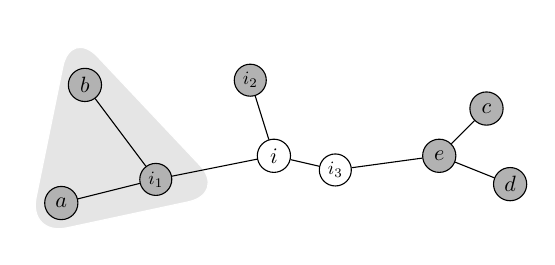
\begin{tikzpicture}[scale=.6]
 \draw[rounded corners=5mm, fill=gray!20, draw=white] (-.7,-.2) -- (3.5,0.7) -- (0.2,4.2) -- cycle;
 \begin{scope}[every node/.style={circle,draw=black,fill=gray!60,minimum size=1.5em, inner sep=2, scale=.8}]
  \node (a) at (0,0.5) {$a$};
  \node (b) at (0.5,3) {$b$};
  \node (c) at (9,2.5) {$c$};
  \node (d) at (9.5,0.9) {$d$};
  \node[scale=.85] (i1) at (2,1) {$i_1$};
  \node[scale=.85] (i2) at (4,3.1) {$i_2$};
  \node[scale=.85,fill=none] (i3) at (5.8,1.2) {$i_3$};
  \node[fill=none] (i) at (4.5,1.5) {$i$};
  \node (e) at (8,1.5) {$e$};
 \end{scope}
 \draw (a) -- (i1) -- (b);
 \draw (i1) -- (i) -- (i3) -- (e) -- (c);
 \draw (e) -- (d);
 \draw (i) -- (i2);
\end{tikzpicture}
\caption{A multicast tree illustrating the cost contribution from node $i$ to the objective function.
	 Destinations and Steiner nodes are denoted by filled and empty circles, respectively.}
\label{fig:objexp}
\end{figure}

In more general terms, let $T\subseteq G$ be a multicast tree, and let $i\in V_T$ be a node with at least two neighbors in $T$.
For multicasting a message, the power to be assigned to node $i$ is either $p_{ii_1}$ or $p_{ii_2}$, where $i_1$ and $i_2$ are neighbors of $i$ such that
$p_{ii_1}>p_{ii_2}>p_{ij}$ for all other neighbors $j\neq i_1,i_2$ of $i$ in $V_T$.
If the path from the message source to $i$ intersects $i_1$, then power $p_{ii_2}$ is sufficient.
Otherwise, the power $p_{ii_1}$ is required.
At a leaf $i$ with neighbor $i_1$ in $T$, the power assignment is $p_{ii_1}$ if $i$ also is the message source, and zero otherwise.

All nodes in $D$ are assumed to be equally likely to initiate a message.
The frequency at which power levels $p_{ii_1}$ and $p_{ii_2}$ (let $p_{ii_2}=0$ if $i$ is a leaf) are required,
is thus proportional to the number of sources in $D$ that utilize the respective arc for message forwarding.
In the example in Fig.\ \ref{fig:objexp}, the expected power consumption at node $i$ is thus proportional to $4p_{ii_1} + 3p_{ii_2}$.
Summing over all nodes yields the total cost of the tree.

The cost model outlined above aims for minimization of the transmission energy.
As pointed out by \citet{halgamuge}, transmission constitutes a substantial part of the total energy consumption in wireless sensor networks.
The energy consumed by other operations, such as sensing, logging, processing, actuation, and cluster formation is less sensitive to the topology
of the multicast tree, and is neglected in the current work.
This is in line with the approach taken in the wide range of literature on optimization models for wireless networks mentioned in Section \ref{sec:literature}.
For a detailed energy model for wireless sensor networks, the reader is referred to the article by \citet{halgamuge}.

\subsection{Problem definition} \label{sec:probdef}

To express the cost of the multicast tree more rigorously, let $T^s=(V_T,A^s)$ denote the directed tree (arborescence) obtained by directing all edges in $T$ such that they point away from the \emph{root} at $s$.
For each arc $(i,j)\in A$, we let $n_{ij}(T)$ denote the number of destinations $s$ such that $(i,j)$ is the most expensive arc leaving node $i$ in $T^s$.
That is,
\[
  n_{ij}(T) = \left|\left\{s\in D: p_{ij}=\max_{k\in V_i: (i,k)\in A^s}p_{ik}\right\}\right|,
\]

\noindent
and the total cost of tree $T$ becomes:
$$
  c(T) = \sum_{i\in V_T}\sum_{j\in V_T:\{i,j\}\in E_T}p_{ij}n_{ij}(T).
$$ 
The problem under study is thus defined in network optimization terms:

\begin{problem}
\label{def:problem}
\textsc{Minimum Shared Multicast Tree}: Find a tree $T\subseteq G$ spanning $D$ such that $c(T)$ is minimized.
\end{problem}

While the feasible domains of the \textsc{Minimum Steiner Tree} problem and SMT are identical,
the cost functions differ.
In the former problem, all edges present in the tree contribute to the objective function by a cost that is given by the input data.
The input cost factor $p_{ij}$ is, in the case of SMT, scaled by a topology dependent factor $n_{ij}(T)$.
Only edges that are the most or second-most expensive edge incident to either of their end nodes get a positive scaling factor.
Some edges in $T$ can thus be scaled down to zero cost, while the most expensive ones are scaled up.

Problem \ref{def:problem} also has close resemblance with the SBT problem, which is the special case of SMT where $D=V$.
Like many other network design problems, SMT is NP-hard.
This follows directly from the NP-hardness of SBT \citep{Papadimitriou06SBT}.


In the forthcoming sections, we develop and analyze IP models for SMT.
All formulations under study are extensions of models previously developed for the related problems mentioned above.
